% Options for packages loaded elsewhere
\PassOptionsToPackage{unicode}{hyperref}
\PassOptionsToPackage{hyphens}{url}
%
\documentclass[
]{article}
\usepackage{amsmath,amssymb}
\usepackage{iftex}
\ifPDFTeX
  \usepackage[T1]{fontenc}
  \usepackage[utf8]{inputenc}
  \usepackage{textcomp} % provide euro and other symbols
\else % if luatex or xetex
  \usepackage{unicode-math} % this also loads fontspec
  \defaultfontfeatures{Scale=MatchLowercase}
  \defaultfontfeatures[\rmfamily]{Ligatures=TeX,Scale=1}
\fi
\usepackage{lmodern}
\ifPDFTeX\else
  % xetex/luatex font selection
\fi
% Use upquote if available, for straight quotes in verbatim environments
\IfFileExists{upquote.sty}{\usepackage{upquote}}{}
\IfFileExists{microtype.sty}{% use microtype if available
  \usepackage[]{microtype}
  \UseMicrotypeSet[protrusion]{basicmath} % disable protrusion for tt fonts
}{}
\makeatletter
\@ifundefined{KOMAClassName}{% if non-KOMA class
  \IfFileExists{parskip.sty}{%
    \usepackage{parskip}
  }{% else
    \setlength{\parindent}{0pt}
    \setlength{\parskip}{6pt plus 2pt minus 1pt}}
}{% if KOMA class
  \KOMAoptions{parskip=half}}
\makeatother
\usepackage{xcolor}
\usepackage[margin=1in]{geometry}
\usepackage{longtable,booktabs,array}
\usepackage{calc} % for calculating minipage widths
% Correct order of tables after \paragraph or \subparagraph
\usepackage{etoolbox}
\makeatletter
\patchcmd\longtable{\par}{\if@noskipsec\mbox{}\fi\par}{}{}
\makeatother
% Allow footnotes in longtable head/foot
\IfFileExists{footnotehyper.sty}{\usepackage{footnotehyper}}{\usepackage{footnote}}
\makesavenoteenv{longtable}
\usepackage{graphicx}
\makeatletter
\def\maxwidth{\ifdim\Gin@nat@width>\linewidth\linewidth\else\Gin@nat@width\fi}
\def\maxheight{\ifdim\Gin@nat@height>\textheight\textheight\else\Gin@nat@height\fi}
\makeatother
% Scale images if necessary, so that they will not overflow the page
% margins by default, and it is still possible to overwrite the defaults
% using explicit options in \includegraphics[width, height, ...]{}
\setkeys{Gin}{width=\maxwidth,height=\maxheight,keepaspectratio}
% Set default figure placement to htbp
\makeatletter
\def\fps@figure{htbp}
\makeatother
\setlength{\emergencystretch}{3em} % prevent overfull lines
\providecommand{\tightlist}{%
  \setlength{\itemsep}{0pt}\setlength{\parskip}{0pt}}
\setcounter{secnumdepth}{-\maxdimen} % remove section numbering
\usepackage{titlesec}
\titleformat*{\section}{\normalfont\Large\bfseries\flushleft}
\titleformat*{\subsection}{\normalfont\large\bfseries\flushleft}
\titleformat*{\subsubsection}{\normalfont\normalsize\bfseries\flushleft}
\usepackage{amsmath}
\newcommand*{\defeq}{\mathrel{\vcenter{\baselineskip0.5ex \lineskiplimit0pt \hbox{\scriptsize.}\hbox{\scriptsize.}}}=}
\newcommand*{\eqdef}{=\mathrel{\vcenter{\baselineskip0.5ex \lineskiplimit0pt \hbox{\scriptsize.}\hbox{\scriptsize.}}}}
\ifLuaTeX
  \usepackage{selnolig}  % disable illegal ligatures
\fi
\IfFileExists{bookmark.sty}{\usepackage{bookmark}}{\usepackage{hyperref}}
\IfFileExists{xurl.sty}{\usepackage{xurl}}{} % add URL line breaks if available
\urlstyle{same}
\hypersetup{
  pdftitle={Statistical Learning (5454) - Assignment 2},
  pdfauthor={Matthias Hochholzer, Lukas Pirnbacher, Anne Valder},
  hidelinks,
  pdfcreator={LaTeX via pandoc}}

\title{Statistical Learning (5454) - Assignment 2}
\author{Matthias Hochholzer, Lukas Pirnbacher, Anne Valder}
\date{Due: 2024-04-22}

\begin{document}
\maketitle

\hypertarget{exercise-1}{%
\section{Exercise 1}\label{exercise-1}}

After generating the simulated data, we fit four models using least
squares. We then calculate the AIC values and determine the in-sample
error estimates by drawing suitable test data from the data generating
process using twice the negative log-likelihood as loss function.

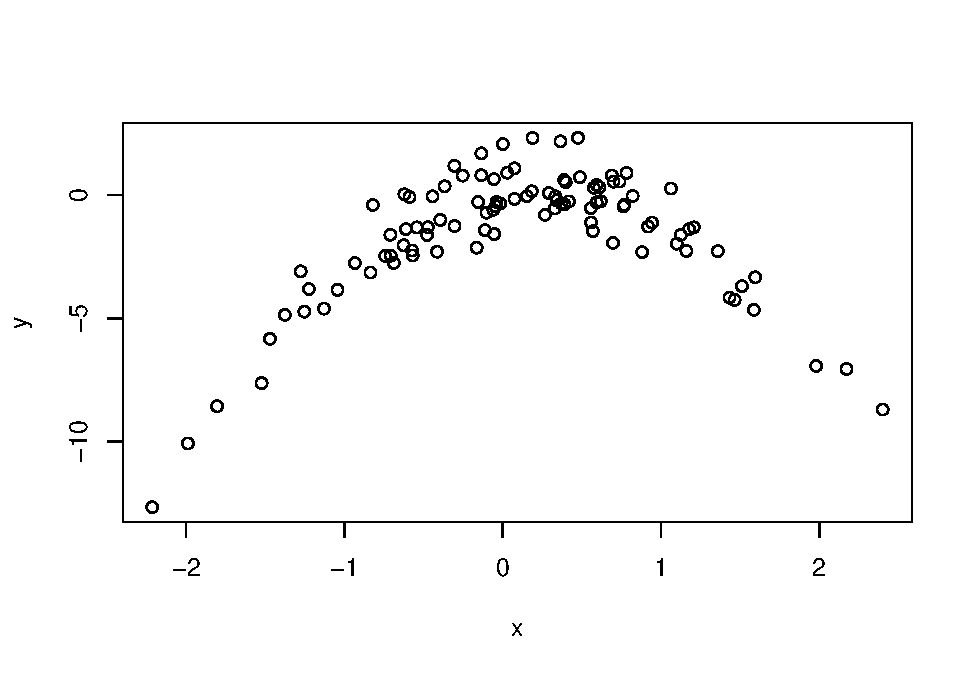
\includegraphics{A2_files/figure-latex/unnamed-chunk-3-1.pdf}

\begin{verbatim}
## [1] "AIC:"
\end{verbatim}

\begin{verbatim}
##       linear    quadratic        cubed fourth_power 
##     478.8804     280.1670     282.0886     282.2963
\end{verbatim}

Plotting the simulated data, we see a clearly non-linear relationship
between \(x\) and \(y\). In line with this, we observe that the linear
specification (model 1) performs worst according to the AIC. The most
preferable model in terms of AIC value is the second model, closely
followed by models 3 and 4.

We now want to compute estimates of the in-sample error \[
\text{Err}_{\text{in}} = \frac{1}{N} \sum_{i=1}^N \mathbb{E}\left[ L\left(y,\hat{f}(x_i)\right) \Big| \mathcal{T}\right],
\] where the expectation is over the distribution of \(y\) given \(x_i\)
and twice the negative log-likelihood is used as loss function. We
approximate the expectations by computing means. To do so, we sample
\(N_{\text{error}}=1000\) error terms for each data point and then
compute the corresponding new responses
\(y_{i,j} = \hat{f}(x_i) + \epsilon_j, \ j = 1,\ldots, 1000\).

In order to evaluate the likelihood function of \(y\), we need estimates
of the error variance \(\sigma^2\), i.e.~the conditional variance of
\(y\) given \(x_i\). We consider both the MLE estimator of \(\sigma^2\)
(which is used in the R implementation of the function \textit{AIC()})
and the unbiased estimator that corrects for the degrees of freedom.

\begin{verbatim}
## [1] "MLE estimator of error variance:"
\end{verbatim}

\begin{verbatim}
## $linear
## in_sample_error             aic 
##        3.880820        4.788804 
## 
## $quadratic
## in_sample_error             aic 
##        2.847452        2.801670 
## 
## $cubed
## in_sample_error             aic 
##        2.839417        2.820886 
## 
## $fourth_power
## in_sample_error             aic 
##        2.845200        2.822963
\end{verbatim}

\begin{verbatim}
## [1] "Unbiased estimator of error variance:"
\end{verbatim}

\begin{verbatim}
## $linear
## in_sample_error             aic 
##        3.879415        4.788804 
## 
## $quadratic
## in_sample_error             aic 
##        2.845433        2.801670 
## 
## $cubed
## in_sample_error             aic 
##        2.841277        2.820886 
## 
## $fourth_power
## in_sample_error             aic 
##        2.849490        2.822963
\end{verbatim}

We find that models 2 to 4 have very similar in-sample errors. For those
models, the discrepancy between our in-sample error estimates and the
AIC values are rather small. The linear specification yields by far the
largest in-sample error and also the gap between the estimated in-sample
error and AIC is quite pronounced, which might be due to model
misspecification.

\hypertarget{exercise-2}{%
\section{Exercise 2}\label{exercise-2}}

In exercise 2, we perform leave-one-out cross-validation (LOOCV),
\(k\)-fold cross-validation (\(k\)CV) and empirical bootstrapping based
on the mean squared error loss that results from fitting the four models
using least squares. The simulated data and specifications are the same
as in task 1. The results of task (b) across the models are shown in
table 1, indicated by ``seed1'' in the last column.

\begin{enumerate}
\def\labelenumi{(\alph{enumi})}
\setcounter{enumi}{2}
\tightlist
\item
  Next, we repeat (b) using another random seed (indicated by ``seed2''
  in table 1). For LOOCV we obtain exactly the same results for all four
  models regardless of the different seed. This is because in general
  the randomness lies in the data generation.This consistency is
  expected because LOOCV is deterministic in this context, not relying
  on random sampling. Each observation is used once as a test set while
  the rest are used for training, and this process is repeated for each
  observation in the dataset. Therefore, changing the seed does not
  affect LOOCV results. For \(k\)CV we observe slight differences in the
  errors between seed 1 and seed 2 across the models. This variation can
  be attributed to the random partitioning of the data into \(k\) folds.
  Each seed leads to a different random split, which can result in
  slight variations in the training and validation sets used in each
  fold, thus affecting the error estimates. Similar to \(k\)CV, the
  bootstrap error shows variations between the two seeds. Bootstrap
  resampling involves drawing samples with replacement from the original
  data set to create ``new'' data sets. The randomness introduced by the
  seed affects which observations are selected in each resample, leading
  to slight differences in the bootstrap error estimates between seed 1
  and seed 2.
\end{enumerate}

\begin{longtable}[]{@{}lrrrll@{}}
\caption{Comparison of LOOCV, kCV, and Bootstrap Errors}\tabularnewline
\toprule\noalign{}
& LOOCV & kCV & Bootstrap & Model & Seed \\
\midrule\noalign{}
\endfirsthead
\toprule\noalign{}
& LOOCV & kCV & Bootstrap & Model & Seed \\
\midrule\noalign{}
\endhead
\bottomrule\noalign{}
\endlastfoot
1 & 7.2882 & 6.1856 & 6.2931 & Model 1 & Seed1 \\
5 & 7.2882 & 6.4165 & 6.2764 & Model 1 & Seed2 \\
2 & 0.9374 & 0.9230 & 0.8702 & Model 2 & Seed1 \\
6 & 0.9374 & 0.9012 & 0.8704 & Model 2 & Seed2 \\
3 & 0.9566 & 0.9316 & 0.8554 & Model 3 & Seed1 \\
7 & 0.9566 & 0.8854 & 0.8557 & Model 3 & Seed2 \\
4 & 0.9539 & 0.9247 & 0.8393 & Model 4 & Seed1 \\
8 & 0.9539 & 0.8962 & 0.8452 & Model 4 & Seed2 \\
\end{longtable}

\begin{enumerate}
\def\labelenumi{(\alph{enumi})}
\setcounter{enumi}{3}
\item
  The MSEs in table 1 suggest that according to LOOCV the second model
  is the best. With \(k\)CV the third model is the best and for the
  empirical bootstrap error it is the fourth model. Also, we see that
  the empirical bootstrap error decreases further with model complexity,
  reflecting potential overfitting problems of this method. Remembering
  the plotted data in the beginning, these results are in line with our
  expectations since higher order regression equations fit much better
  to the data than the linear case.
\item
  Last, we have a look at the statistical significance of the
  coefficient estimates that result from fitting each of the models
  using least squares. The results here align with our previous
  conclusions, in the sense that the quadratic term has the lowest
  p-value. At the same time, none of the coefficients corresponding to
  the higher-order terms in models 3 and 4 are statistically significant
  at a 5\% or even 10\% level. Thus, while the more complex models
  performed well in terms of \(k\)CV and empirical bootstrapping errors,
  model selection based on \(t\)-tests for the individual coefficients
  rejects them.
\end{enumerate}

\begin{verbatim}
## [[1]]
##              Estimate Std. Error   t value     Pr(>|t|)
## (Intercept) -1.625427  0.2619366 -6.205420 1.309300e-08
## x            0.692497  0.2909418  2.380191 1.923846e-02
## 
## [[2]]
##                Estimate Std. Error    t value     Pr(>|t|)
## (Intercept)  0.05671501  0.1176555   0.482043 6.308613e-01
## x            1.01716087  0.1079827   9.419666 2.403287e-15
## I(x^2)      -2.11892120  0.0847657 -24.997388 4.584330e-44
## 
## [[3]]
##                Estimate Std. Error     t value     Pr(>|t|)
## (Intercept)  0.06150718 0.11950374   0.5146883 6.079538e-01
## x            0.97528027 0.18728149   5.2075636 1.089350e-06
## I(x^2)      -2.12379099 0.08700251 -24.4106856 5.873444e-43
## I(x^3)       0.01763858 0.06429037   0.2743580 7.843990e-01
## 
## [[4]]
##                 Estimate Std. Error     t value     Pr(>|t|)
## (Intercept)  0.156702953 0.13946192   1.1236253 2.640034e-01
## x            1.030825643 0.19133655   5.3874999 5.174326e-07
## I(x^2)      -2.409898183 0.23485506 -10.2612148 4.575229e-17
## I(x^3)      -0.009132904 0.06722881  -0.1358481 8.922288e-01
## I(x^4)       0.069785421 0.05324006   1.3107691 1.930956e-01
\end{verbatim}

\hypertarget{exercise-3}{%
\section{Exercise 3}\label{exercise-3}}

Here we are using the wage data set available as data object
\(\textit{Schooling}\) in package \(\textbf{Ecda}\). First, we omit
observations with missing values and the variable wage76, and mutate
variable mar76 into a binary variable. Next, we fit regularized linear
regression models with lwage76 as dependent variable using only linear
effects for the covariates and varying the \(\alpha\) parameter for the
elastic from 0 to 1 in step sizes of 0.2. We do this using using the
function \textit{cv.glmnet} with 10-fold cross-validation, considering
the MSE for a range of penalty values of \(\lambda\). The argument
``foldid'' ensures that the same data partitions are used for each model
fitting, making the comparisons fair and consistent. The default plot
method for \textit{cv.glmnet} objects is used to visualize the
cross-validation curves, which show the mean squared error (MSE) across
a range of \(\lambda\) values for each \(\alpha\). The plots display the
\(\lambda\) values on the log scale along the bottom \(x\)-axis and the
corresponding MSE on the \(y\)-axis. The vertical dotted line on the
left in each plot indicates the \(\lambda\) value that gives the minimum
MSE.

By varying \(\alpha\), we essentially move between different
regularization methods: \(\alpha = 0\) corresponds to ridge regression
(penalty on the square of coefficients), \(\alpha = 1\) corresponds to
lasso regression (penalty on the absolute value of coefficients). The
top \(x\)-axis shows these numbers, which correspond to the model's
complexity at different levels of regularization. As \(\lambda\)
increases, the regularization penalty becomes more severe, leading to
more coefficients being shrunk to zero. The dual \(x\)-axes in the plot
serve to simultaneously convey how \(\lambda\) affects both the model's
predictive accuracy (through the MSE shown on the \(y\)-axis) and its
complexity (in terms of the number of predictors used, shown on the
bottom \(x\)-axis).

Looking at the different plots, given each value of \(\alpha\), we
observe with \(\alpha\) closer to 1 more pronounced changes in the
number of non-zero coefficients as \(\lambda\) changes, reflecting the
lasso's variable selection property. For ridge regression
(\(\alpha = 0\)), the coefficients are shrunk towards zero but not
exactly to zero, so the model complexity in terms of the non-zero
coefficient count may not reduce as dramatically as with lasso or
elastic net. The visualization helps in choosing an optimal \(\lambda\)
value, typically via the 1-standard error rule or by selecting the value
of \(\lambda\) that minimizes the cross-validation error.

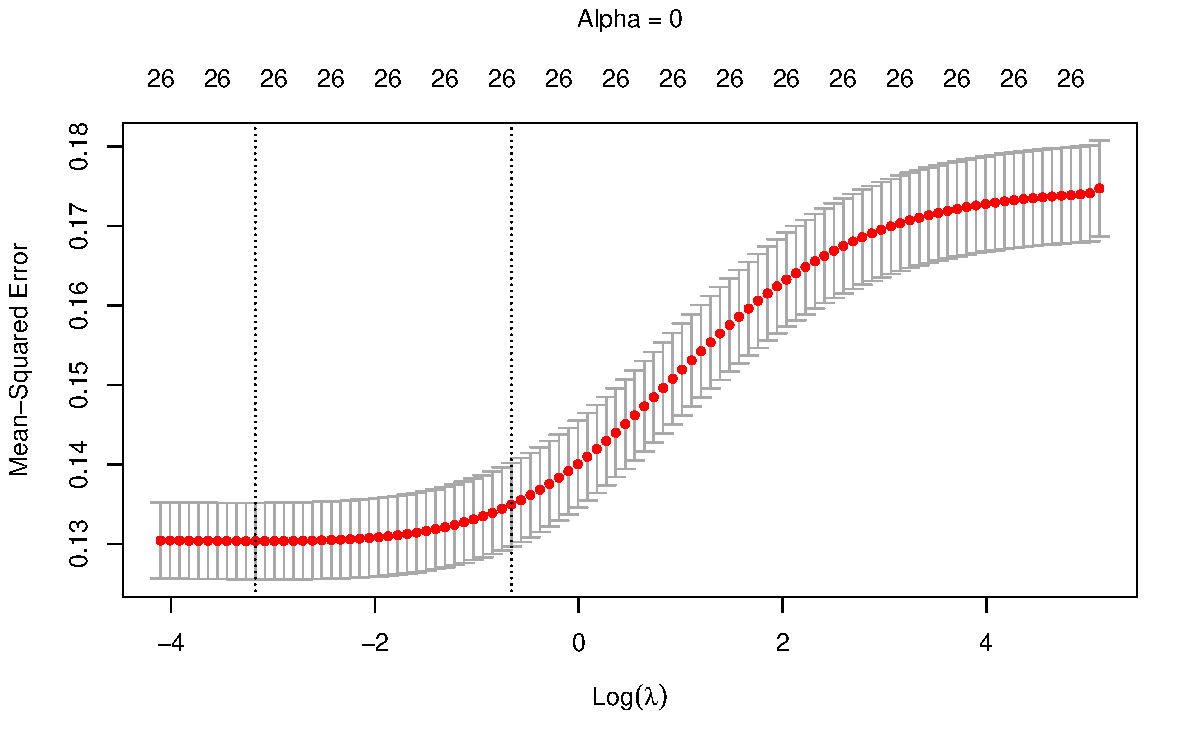
\includegraphics{A2_files/figure-latex/unnamed-chunk-8-1.pdf}
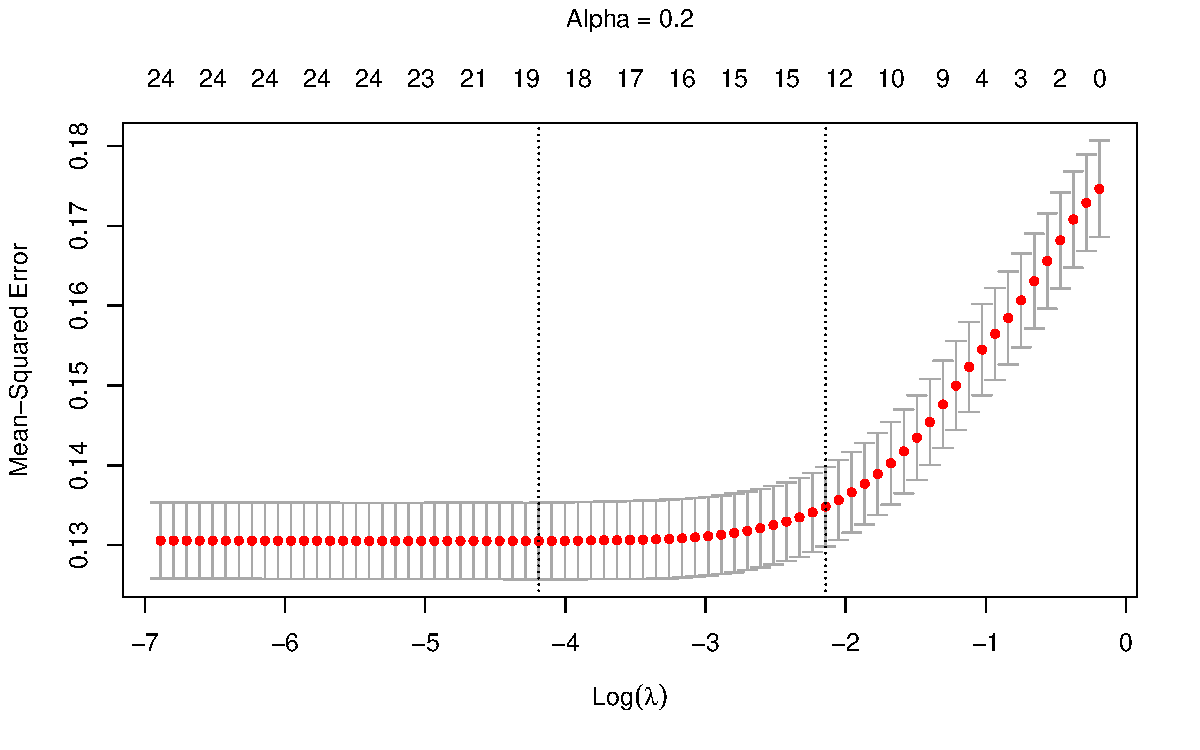
\includegraphics{A2_files/figure-latex/unnamed-chunk-8-2.pdf}
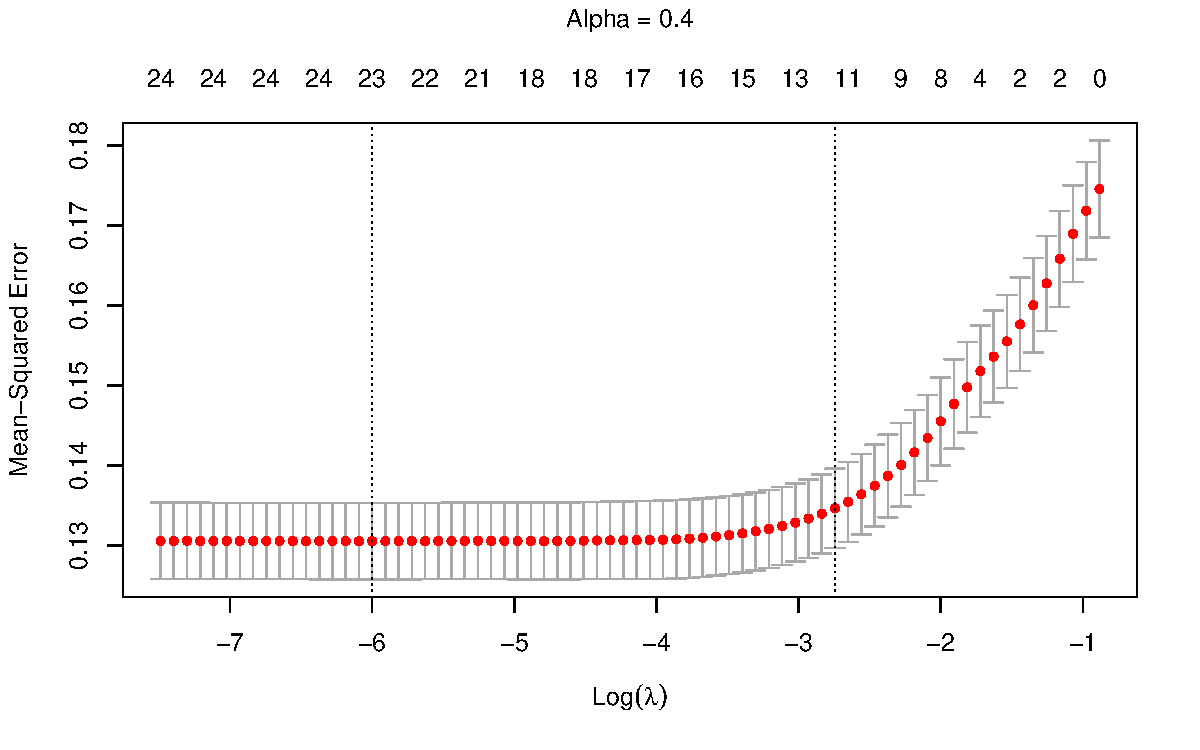
\includegraphics{A2_files/figure-latex/unnamed-chunk-8-3.pdf}
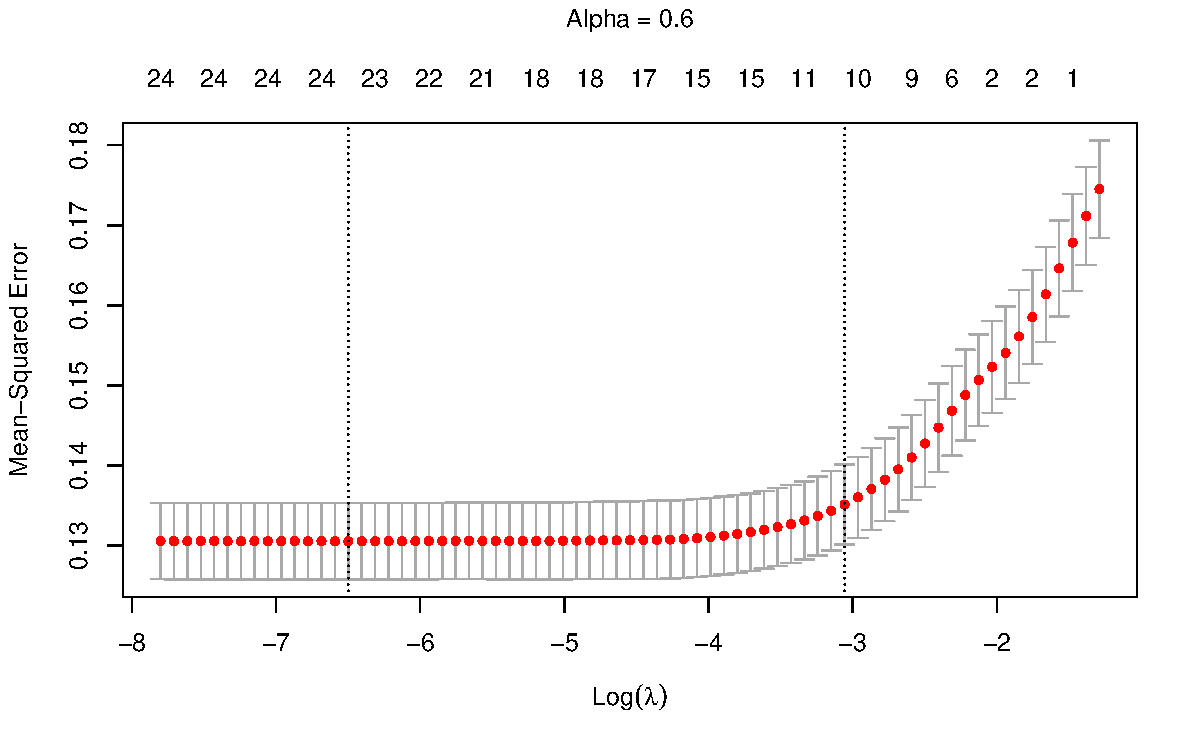
\includegraphics{A2_files/figure-latex/unnamed-chunk-8-4.pdf}
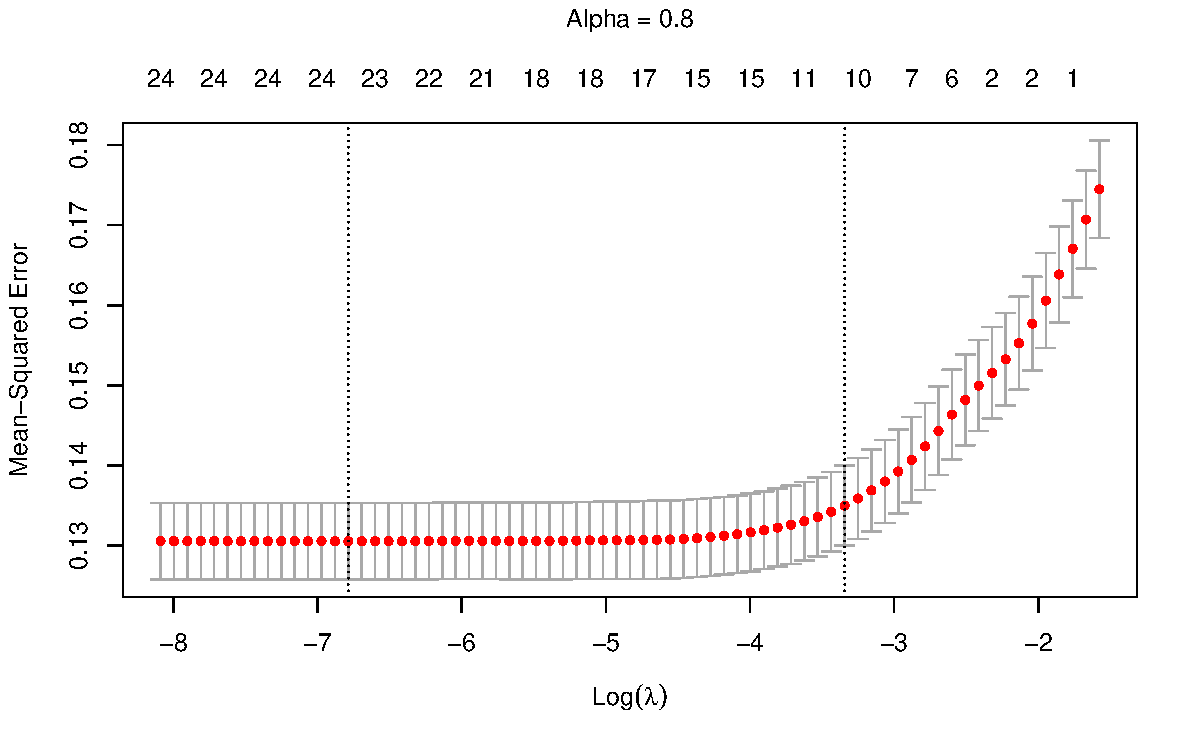
\includegraphics{A2_files/figure-latex/unnamed-chunk-8-5.pdf}
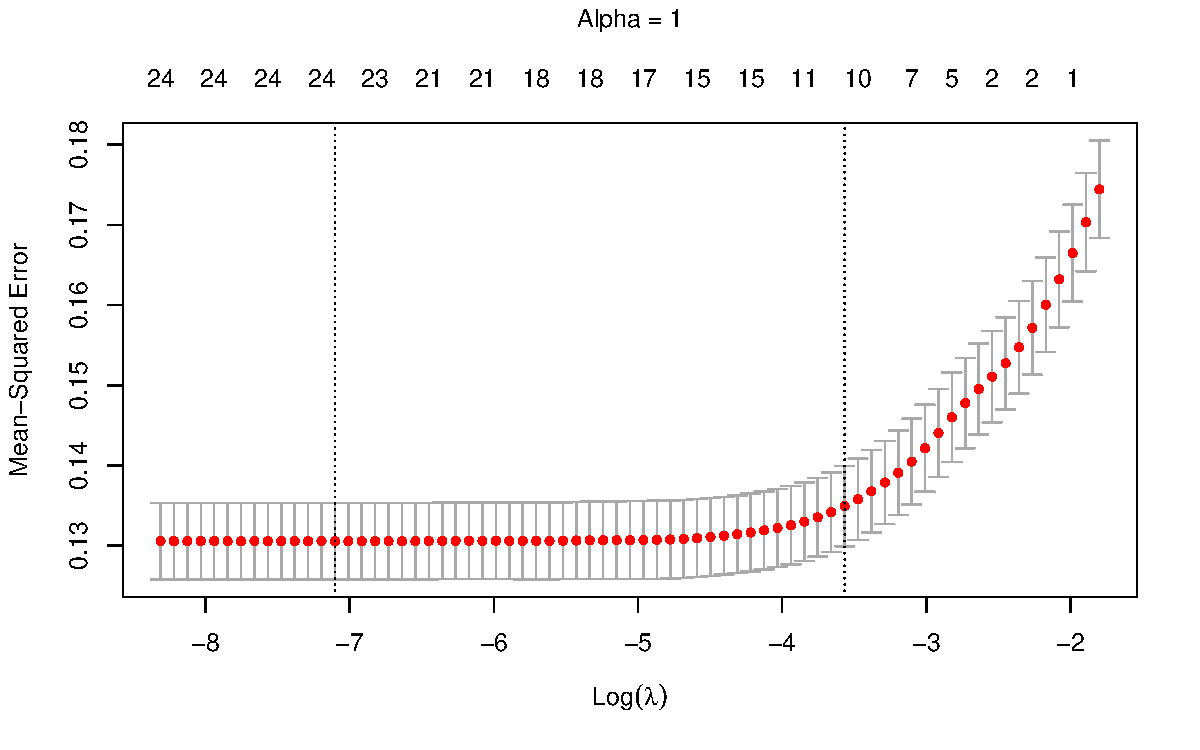
\includegraphics{A2_files/figure-latex/unnamed-chunk-8-6.pdf}

Next, to select the best value for \(\lambda\), that balances model
simplicity and accuracy, for each fixed value of \(\alpha\) we look at
either the value that minimizes the cross-validation error (lambda.min)
or the 1-SE rule (lambda.1se), and then compare the selected models. We
extract these \(\lambda\) values from \textit{cv.glmnet} and then fit
the final models on the full data set using these selected \(\lambda\)
value. To compare the selected models based on their complexity (number
of non-zero coefficients), predicted values and MSE, we can use the
\textit{coef} function to inspect the coefficients, make predictions
with the \textit{predict} function and then calculate MSE for each
model.

Table 2 summarizes all that. The choice between lambda.min and
lambda.1se involves a trade-off between model simplicity and predictive
accuracy. lambda.1se typically leads to simpler models (with potentially
slightly higher MSE). We observe that as \(\alpha\) increases from 0 to
1, the number of non-zero coefficients varies. The model with
\(\alpha = 0\) (ridge regression) maintains 27 non-zero coefficients for
both lambda.min and lambda.1se. For other values of \(\alpha\) (moving
towards lasso regression), the number of non-zero coefficients tends to
decrease, indicating sparser models. This is especially visible for
\(\alpha = 1.0\) with only 11 non-zero coefficients in case of
lambda.1se, suggesting that lasso regularization enforces the most
sparsity.

Regarding predicted values, the CV MSE does not vary significantly
across different \(\alpha\) values, indicating that the change in
\(\alpha\) is not drastically affecting the model's predictive ability
in this case. The lowest CV MSE for lambda.min appears at
\(\alpha = 0\), suggesting that the ridge model at its optimal
\(\lambda\) achieves a marginally better fit in terms of MSE. For the
lambda.1se criterion, the CV MSE is slightly higher compared to
lambda.min, which is expected as the 1-SE rule tends to select a simpler
and more generalizable model at the expense of a slight increase in
error. In the end, the choice between lambda.min and lambda.1se would
depend on whether the priority is on the lowest possible MSE or on model
simplicity.

\begin{longtable}[]{@{}rrlrr@{}}
\toprule\noalign{}
alpha & lambda & criterion & non\_zero\_coefficients & cv\_mse \\
\midrule\noalign{}
\endhead
\bottomrule\noalign{}
\endlastfoot
0.0 & 0.0419448 & min & 27 & 0.1303431 \\
0.0 & 0.5171153 & 1se & 27 & 0.1349293 \\
0.2 & 0.0151438 & min & 19 & 0.1304989 \\
0.2 & 0.1172527 & 1se & 13 & 0.1348111 \\
0.4 & 0.0024795 & min & 24 & 0.1305440 \\
0.4 & 0.0643424 & 1se & 12 & 0.1346541 \\
0.6 & 0.0015061 & min & 25 & 0.1305523 \\
0.6 & 0.0470771 & 1se & 12 & 0.1351290 \\
0.8 & 0.0011296 & min & 24 & 0.1305559 \\
0.8 & 0.0353078 & 1se & 12 & 0.1349972 \\
1.0 & 0.0008234 & min & 24 & 0.1305582 \\
1.0 & 0.0282463 & 1se & 11 & 0.1349284 \\
\end{longtable}

Last, we inspect the best solution for \(\alpha = 1\) (lasso regression)
using the 1-SE rule. This approach tends to prefer simpler models with
fewer non-zero coefficients, which can be advantageous for
interpretability and generalization. To see which variables were
selected (i.e., have non-zero coefficients) and their estimated
coefficients, we use the \textit{coef} function from the \textbf{glmnet}
package. We observe that only 10 variables (plus the intercept) are
selected and that all of them have rather small coefficients and thus
little influence on the response variable `lwage76'.

\begin{verbatim}
## [1] "Non-zero coefficients (including intercept):"
\end{verbatim}

\begin{verbatim}
## 27 x 1 sparse Matrix of class "dgCMatrix"
##                        s1
## (Intercept)  5.2606230123
## smsa66yes    0.0125799380
## smsa76yes    0.0931998619
## nearc2yes    .           
## nearc4yes    .           
## nearc4ayes   .           
## nearc4byes   .           
## ed76         .           
## ed66         0.0474880207
## age76        0.0060773554
## daded        .           
## nodadedyes   .           
## momed        .           
## nomomedyes   .           
## momdad14yes  .           
## sinmom14yes  .           
## step14yes    .           
## south66yes   .           
## south76yes  -0.0376576668
## famed        .           
## blackyes    -0.0601258292
## enroll76yes -0.0287117356
## kww          0.0055338639
## iqscore      0.0005873908
## mar76TRUE    0.0615223905
## libcrd14yes  .           
## exp76        .
\end{verbatim}

To assess the goodness-of-fit, we calculate the correlation between the
predicted values from the model and the observed values. Values closer
to 1 or -1 indicating a stronger linear relationship between predictions
and actual outcomes. In this case the correlation lies at roughly 0.5.
This indicates a moderate positive linear relationship between the
predicted and observed values. The model therefore has some predictive
power, but it is not capturing all of the variability in the dependent
variable.

\begin{verbatim}
## [1] "Correlation between predicted and observed values for alpha = 1 (1-SE rule): 0.5018"
\end{verbatim}

\newpage

\hypertarget{exercise-4}{%
\section{Exercise 4}\label{exercise-4}}

In this exercise we use the South African heart disease data available
as data object \textit{SAheart} in the package \textbf{Elem-StatLearn}.
We fit a logistic regression model with Lasso penalty using only linear
effects for the covariates and perform 20-fold cross-validation. We
consider the deviance loss function, which is the default in the
\textit{cv.glmnet} function of the \textbf{glmnet} package. Once again,
we visualize the results using the default plot method.

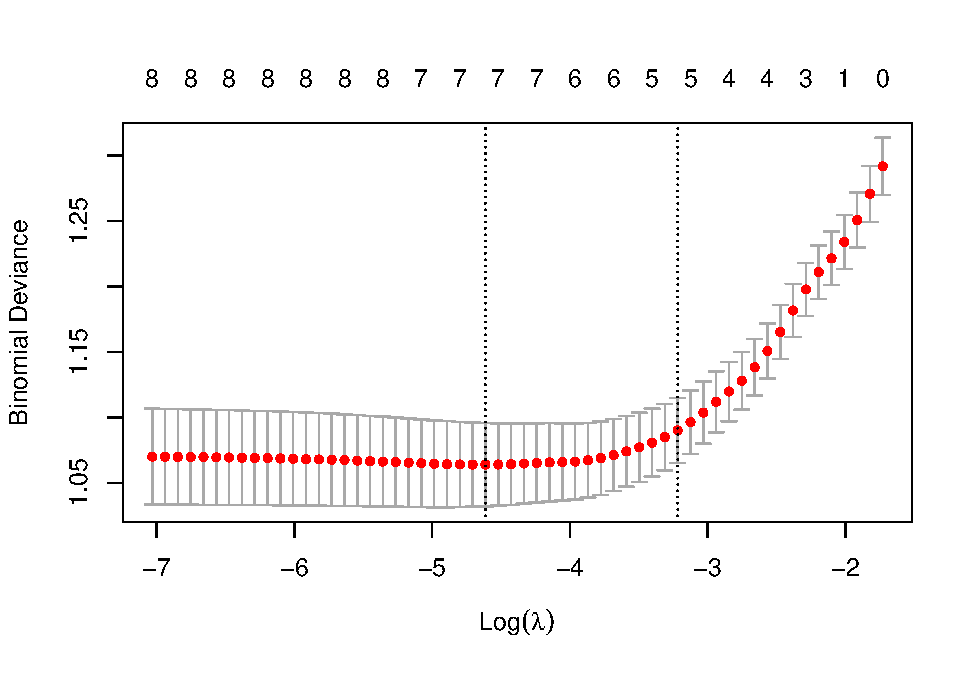
\includegraphics{A2_files/figure-latex/unnamed-chunk-12-1.pdf} Next, we
want to focus on two particular values of the penalty \(\lambda\),
namely the one that minimizes the CV deviance loss and the one based on
the 1-SE rule. These are given by

\begin{verbatim}
## 
## Call:  cv.glmnet(x = X, y = y, nfolds = 20, family = "binomial") 
## 
## Measure: Binomial Deviance 
## 
##      Lambda Index Measure      SE Nonzero
## min 0.00992    32   1.064 0.03188       7
## 1se 0.04005    17   1.090 0.02480       5
\end{verbatim}

We immediately see that lambda.min yields a more complex model (with 7
non-zero coefficients) than lambda.1se (with 5 non-zero coefficients).
Looking at the coefficient estimates, we do find some notable
differences between the two models, especially when it comes to the
effect of `famhistPresent':

\begin{verbatim}
## 10 x 2 sparse Matrix of class "dgCMatrix"
##                 lambda.min   lambda.1se
## (Intercept)    -5.73717333 -3.491091421
## sbp             0.00416794  .          
## tobacco         0.07056290  0.047853360
## ldl             0.14789200  0.090034365
## adiposity       .           .          
## famhistPresent  0.81077289  0.545646456
## typea           0.02967640  0.009027127
## obesity        -0.01618876  .          
## alcohol         .           .          
## age             0.04396417  0.033829963
\end{verbatim}

Using the \textit{predict} function, we can now have a look at the
predicted values of the two models, i.e.~the predicted probabilities of
coronary heart disease. Since we have not distinguished between test and
training data in this exercise, we compute predictions for the whole
sample.

We can summarize the predictive performance of the two models by
comparing the MSE for the whole sample:

\begin{verbatim}
## lambda.min lambda.1se 
##  0.1715463  0.1784160
\end{verbatim}

Since we consider in-sample predictions, it is not very surprising that
the more complex model does better in terms of MSE. Moreover, the MSE
might not be a suitable performance measure in the context of logistic
regression. Hence, we now compare the misclassification rates of the two
models.

\begin{verbatim}
## lambda.min lambda.1se 
##  0.2532468  0.2532468
\end{verbatim}

We find that the two models yield the same misclassification rate
in-sample. On the contrary, they quite drastically differ with respect
to their false-positive and false-negative rates:

\begin{verbatim}
## [1] "False-positive rates:"
\end{verbatim}

\begin{verbatim}
## lambda.min lambda.1se 
##  0.1357616  0.0794702
\end{verbatim}

\begin{verbatim}
## [1] "False-negative rates:"
\end{verbatim}

\begin{verbatim}
## lambda.min lambda.1se 
##    0.47500    0.58125
\end{verbatim}

Overall, we find that the false-positive rates of both models are rather
low, while the false-negative rates are fairly high, especially for the
simpler model corresponding to lambda.1se. This is in line with the
observation that 34.6\% of the individuals in the sample suffer from
coronary heart disease while our models predict a prevalence of 27.1\%
and 19.7\%, respectively.

On a final note, we have so far only considered models trained in the
cross-validation procedure. In general, it seems more appropriate to
re-estimate the models for the selected values of \(\lambda\) using the
full data available. However, in this exercise the resulting differences
in parameter estimates are negligible and the predicted classifications
do not change at all.

\newpage

\hypertarget{exercise-5}{%
\section{Exercise 5}\label{exercise-5}}

We load the acoustic-phonetic continuous speech corpus dataset
\textit{phoneme} from the package \textit{ElemStatLearn}. There are five
classes contained in the dataset. The covariates are log-periodograms of
length 256. In the following two-group classification is performed using
only the classes ``aa'' and ``ao''. Therefore, we subset the data
accordingly.

Afterwards, we visualize the data by plotting the covariate values on
the y-axis and the index on the x-axis using line plots. ``aa'' is
plotted in \textit{magenta} and ``ao'' in \textit{blue}. ``aa'' seems to
have overall slightly higher values than ``ao''.

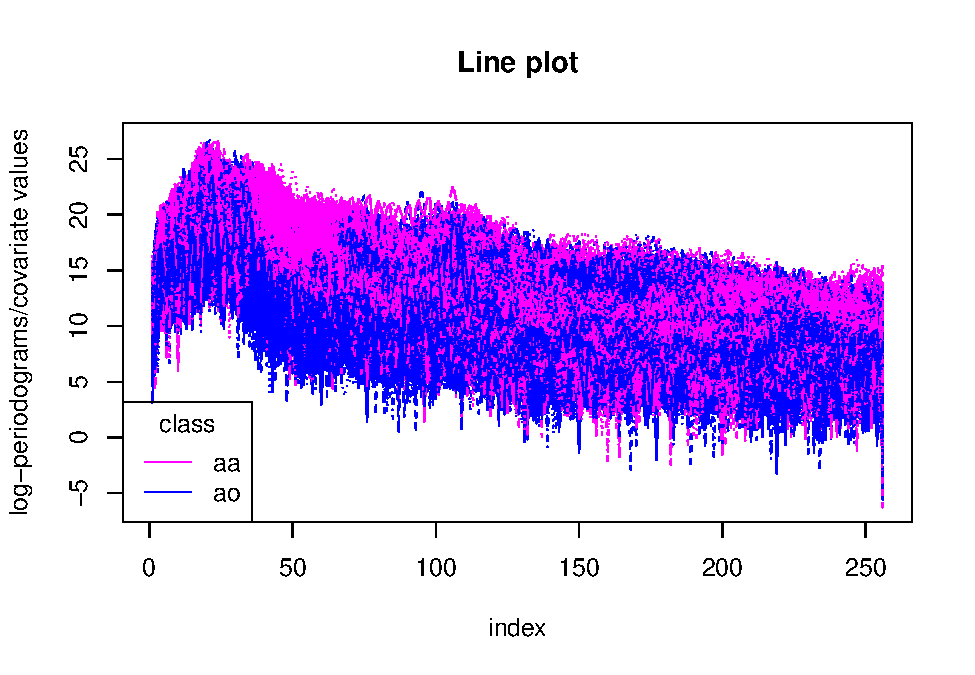
\includegraphics{A2_files/figure-latex/unnamed-chunk-20-1.pdf}

We select 1000 samples as training data and use the remaining ones as
test data.

We then fit a logistic regression model to the training data using all
covariates and determine the misclassification rate and the average
log-likelihood value on the training and test data.

We calculate the average log-likelihood value on the training data in
two ways. The first value is obtained by the \textit{logLik} function.
The second value is obtained via the likelihood function of the
(multivariate) Bernoulli distribution, which is given by
\[\prod_{i=1}^n p^{x_i}(1-p)^{1-x_i}.\] Taking the logarithm gives us
the log-likelihood: \[ \sum_{i=1}^n x_i \log(p)+(1-x_i)\log(1-p). \]

\begin{verbatim}
## 'log Lik.' -0.1927175 (df=257)
\end{verbatim}

\begin{verbatim}
## [1] -0.1927175
\end{verbatim}

Of course, the two approaches yield the same results.

The average log-likelihood value on the test data is calculated with the
second approach.

\begin{verbatim}
## [1] -1.253211
\end{verbatim}

Higher average log-likelihood values speak for a better fit of the
model. Therefore, we also see a lower value for the test data.

To calculate the misclassifications rate we turn the predicted
probabilities into binary outcomes (1 if \(>0.5\), 0 otherwise).
Comparing the prediction to the actual class gives us the
misclassification rate for the training data.

\begin{verbatim}
## [1] 0.068
\end{verbatim}

As well as for the test data.

\begin{verbatim}
## [1] 0.2622036
\end{verbatim}

As expected, the misclassification rate is higher for the test data.

The complexity of this model can be reduced by restricting the
regression coefficients to vary only smoothly over the covariates, i.e.,
regression coefficients for close covariates are similar. To achieve
this, we use splines. We create a 12-dimensional model matrix \(X^*\)
based on natural cubic splines which we use to fit the logistic
regression model instead of the 256-dimensional X. Specifically, we fit
a logistic regression model to the training data using \(X^*\) as model
matrix and determine the misclassification rate and the average
log-likelihood value on the training and test data.

The average log-likelihood value on the training data is calculated as
before.

\begin{verbatim}
## 'log Lik.' -0.3887649 (df=13)
\end{verbatim}

\begin{verbatim}
## [1] -0.3887649
\end{verbatim}

The average log-likelihood value on the test data now is

\begin{verbatim}
## [1] -0.4021256
\end{verbatim}

We observe that by considering splines, the gap between the average
log-likelihood on the test and training data becomes much smaller, which
might be an indication that in this way we avoid overfitting.

For the misclassification rate of the training data we also perform the
same steps as before.

\begin{verbatim}
## [1] 0.164
\end{verbatim}

The misclassification rate of the test data is

\begin{verbatim}
## [1] 0.181311
\end{verbatim}

Hence, we once again conclude that the use of splines in this example
leads to a worse in-sample fit, but a better performance on the test
data.

Next, we vary the degrees of freedom in the spline basis expansion using
2 to the power of 1 to 8, i.e., 2,4,8,16,32,64,128 and 256. Again, we
calculate the misclassifiation rate and the average log-likelihood on
the training and test data for each of the fitted models. We create
helper functions that generalize the steps of the previous
12-dimensional model to \(x\)-dimensional models.

After running the helper functions for all different dimensions of the
spline basis expansion, we are able to compare the misclassification
rates and average log-likelihoods based on training and test data sets
visually for the different degrees of freedom.

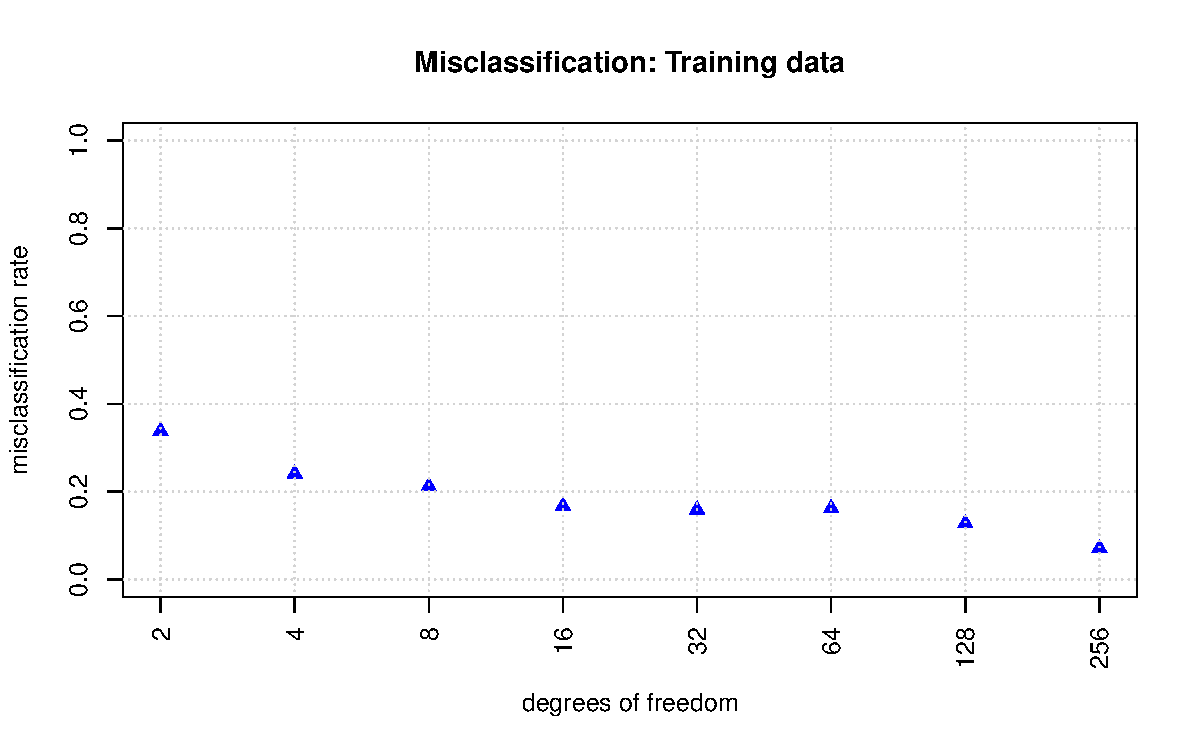
\includegraphics{A2_files/figure-latex/unnamed-chunk-33-1.pdf}
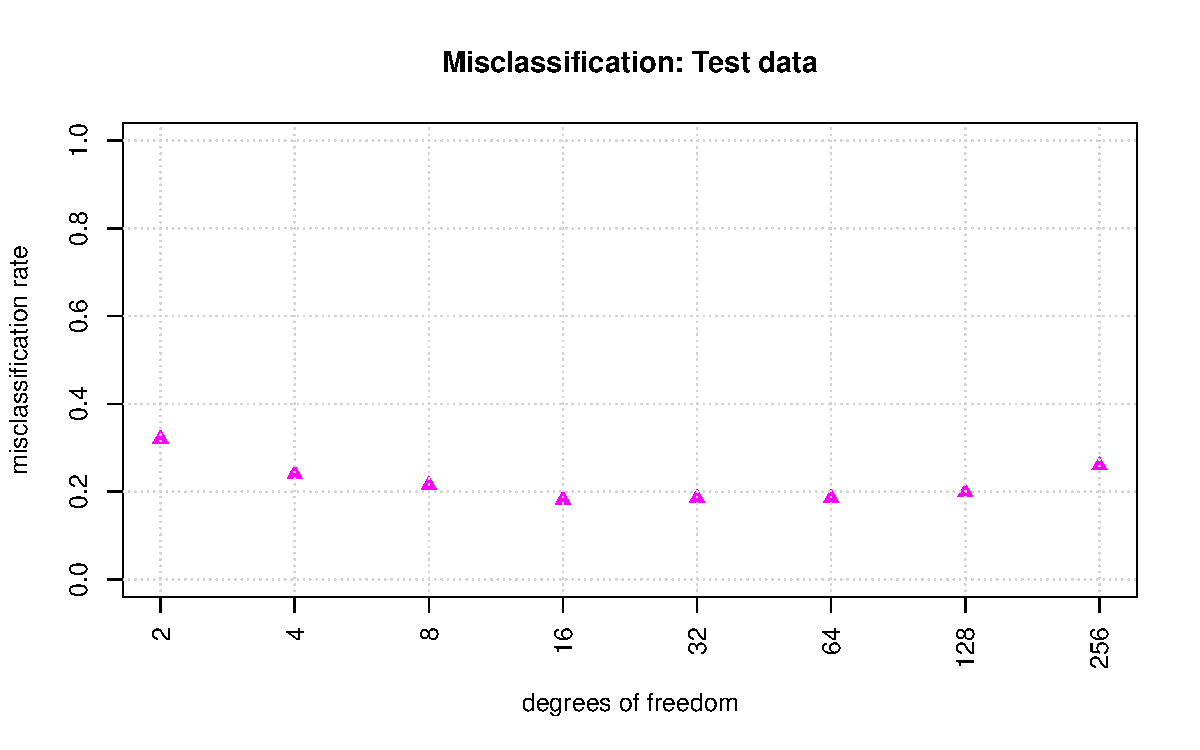
\includegraphics{A2_files/figure-latex/unnamed-chunk-33-2.pdf}
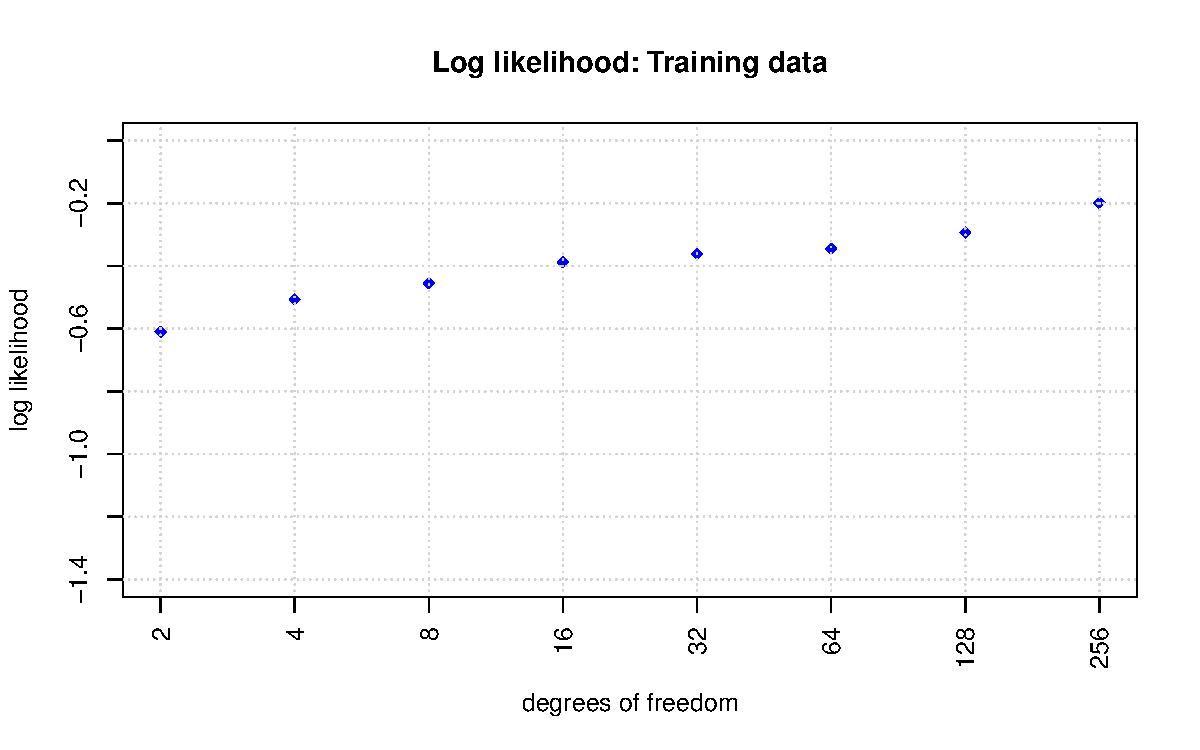
\includegraphics{A2_files/figure-latex/unnamed-chunk-33-3.pdf}
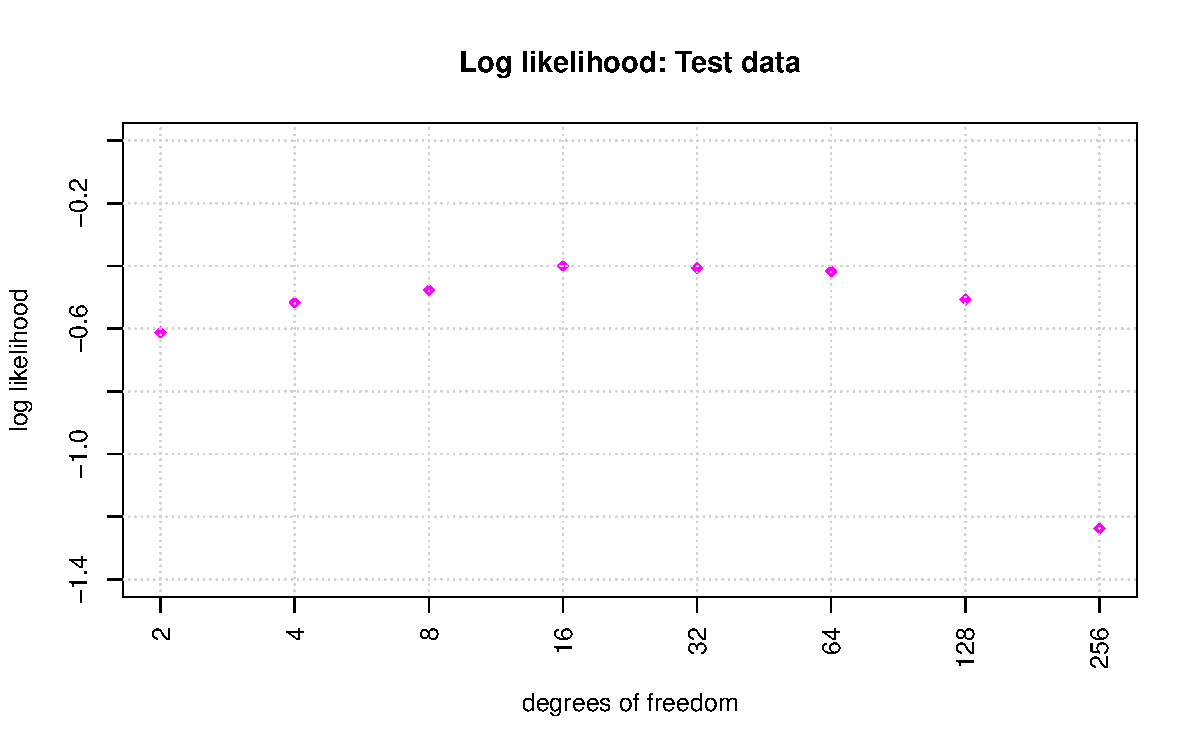
\includegraphics{A2_files/figure-latex/unnamed-chunk-33-4.pdf} The more
we restrict the regression coefficients to vary only smoothly over the
covariates (lower degrees of freedom), the higher is the
misclassification rate for the training data. Theoretically, a higher
degree of smoothing avoids overfitting to the training data. At the same
time, we might lose important information by restricting the
coefficients too much. By looking at the misclassification rate on the
test data, we can see that medium levels of degrees of freedom (16-64)
result in the lowest misclassification rate. Low levels of smoothing, in
other words high degrees of freedom, show the expected overfitting. Too
much smoothing, i.e.~low degrees of freedom, seems to loose important
information and hence also increases the misclassification rate on the
test data.

On the training data, the average log-likelihood increases monotonically
with the degrees of freedom. Hence, the in-sample fit becomes better if
we do not restrict the coefficients to vary smoothly. Looking at the
average log-likelihood on the test data, though, we see that medium
levels of degrees of freedom (16-64) are the best choice. They avoid
overfitting and don't lose too much information either. Note the very
low average log-likelihood due to overiftting for 256 degrees of
freedom. On the other end of the spectrum, with a high level of
smoothing, the loss isn't as pronounced.

\end{document}
